% % % % % Packages % % % % %
\documentclass[11pt]{scrartcl}
\usepackage[sexy]{evan}
\usepackage{imakeidx}
\usepackage{amsmath}
\usepackage{amssymb}
\usepackage{mathtools}
\makeindex[columns=3, title=Alphabetical Index, intoc]
% \usepackage[left=2cm, right=2cm, top=1cm, bottom=2cm]{geometry}
\usepackage{graphicx}
\newcommand*{\rom}[1]{\expandafter\@slowromancap\romannumeral #1@}
% alert -> blue sent
% vocab -> word
% lstlisting
% \begin{lstlisting}[language=C++,basicstyle=\small\ttfamily], [basicstyle=\scriptsize\ttfamily]
% \linespread{1.25}

\newcommand{\mat}[1]{\begin{bmatrix} #1 \end{bmatrix}}

% % % % % Information % % % % %
\title{Ski Resort Database Design}
\author{Group 14: Connor, Luis, Mohammad, Nathan}
\date{Spring 2025}
\hypersetup
{
  pdfauthor={Group 14},
  pdfsubject={HWs CSC 460},
  pdftitle={CSC 460: Homeworks},
}
\begin{document}
\maketitle
\tableofcontents

\section{Conceptual database design}
Figure~\ref{fig:er_diagram} shows the E--R diagram of the ski resort database. 
To design the conceptual schema of the database we first did a detailed walk through fot the program specifications to record what tables are going to be needed to store data. 
The ER diagram we made captures the ski resorts day to day operations tracking members and their activites as well as the resorts staff and income via its services. Attributes
are constrained via sql datatypes.

\begin{figure}[h]
  \centering
  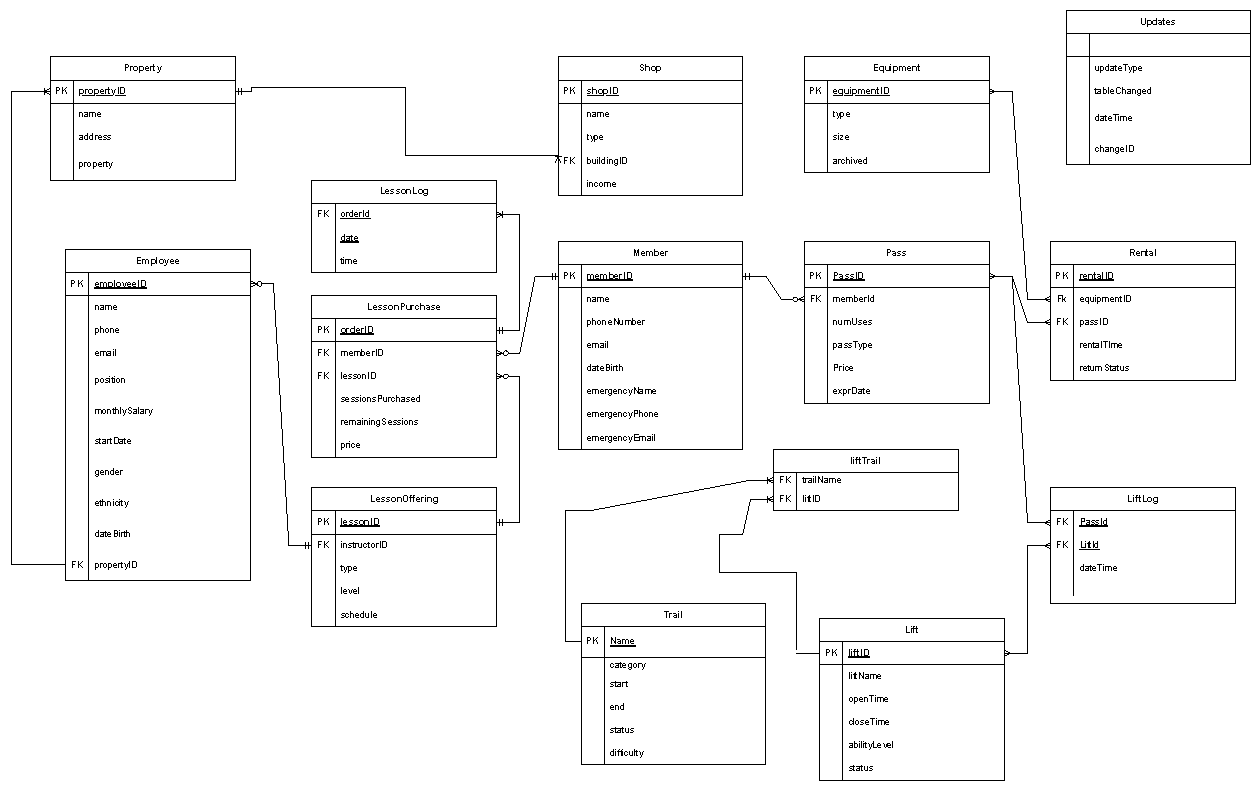
\includegraphics[width=1.1\textwidth]{er.pdf}
  \caption{E--R Diagram of the Ski Resort Database}
  \label{fig:er_diagram}
\end{figure}

\section{Logical database design}

Below is the final relational schema derived from the E--R diagram. Each table lists its attributes, primary keys (\textbf{PK}), and foreign keys (\textbf{FK}) explicitly. 
This design reflects a direct and normalized translation of the conceptual model into the relational model used in Oracle SQL.

\begin{itemize}
  \item \textbf{Property(} \underline{propertyID}, name, address, propertyType \textbf{)}

  \item \textbf{Shop(} \underline{shopID}, name, shopType, buildingID\textsuperscript{FK}, income \textbf{)}

  \item \textbf{Equipment(} \underline{equipmentID}, equipmentType, equipmentSize, archived \textbf{)}

  \item \textbf{Rental(} \underline{rentalID}, equipmentID\textsuperscript{FK}, passID\textsuperscript{FK}, rentalTime, returnStatus \textbf{)}

  \item \textbf{Pass(} \underline{passID}, memberID\textsuperscript{FK}, numUses, passType, price, exprDATE \textbf{)}

  \item \textbf{LiftLog(} passID\textsuperscript{FK}, liftID\textsuperscript{FK}, dateTime \textbf{)}

  \item \textbf{Lift(} \underline{liftID}, liftName, openTime, closeTime, abilityLevel, status \textbf{)}

  \item \textbf{TrailLift(} liftID\textsuperscript{FK}, trailName\textsuperscript{FK} \textbf{)}

  \item \textbf{Trail(} \underline{name}, category, startPos, endPos, status, difficulty \textbf{)}

  \item \textbf{Member(} \underline{memberID}, name, phoneNumber, email, dateBirth, emergencyName, emergencyPhone, emergencyEmail \textbf{)}

  \item \textbf{LessonLog(} orderID\textsuperscript{FK}, dateTime \textbf{)}

  \item \textbf{LessonPurchase(} \underline{orderID}, memberID\textsuperscript{FK}, lessonID\textsuperscript{FK}, sessionsPurchased, remainingSessions, price \textbf{)}

  \item \textbf{LessonOffering(} \underline{lessonID}, instructorID\textsuperscript{FK}, lessonType, skillLevel, schedule \textbf{)}

  \item \textbf{Employee(} \underline{employeeID}, name, phone, email, position, monthlySalary, startDate, gender, ethnicity, dateBirth, propertyID\textsuperscript{FK} \textbf{)}

  \item \textbf{Updates(} updateType, tableChanged, changeID, dateTime \textbf{)}
\end{itemize}

\section{Normalization analysis}

These all adhere to 1NF as all set attributes are non set values. Also, they all adhere to 2NF 
because all non-prime attributes are fully functionally dependant on the candidate keys.

Property( propertyID, name, address, propertyType )
FDs: propertyID -> name, propertyID -> adress, propertyID -> propertyType
This is in BCNF as for all of the FDs X -> Y, X is a superkey (it is the PK)

Shop( shopID, name, type, buildingID, income )
FDs: shopID -> name, shopID -> type, shopID -> buildingID, shopID -> income
This is in BCNF as for all of the FDs X -> Y, X is a superkey (it is the PK)

Equipment( equipmentID, type, size, archived )
FDs: equipmentID -> type, equipmentID -> size, equipmentID -> archived
This is in BCNF as for all of the FDs X -> Y, X is a superkey (it is the PK)

Rental( rentalID, equipmentID, passID, rentalTime, returnStatus )
FDs: rentalID -> equipmentID, rentalID -> passID, rentalID -> rentalTime, rentalID -> rentalStatus
This is in BCNF as for all of the FDs X -> Y, X is a superkey (it is the PK)

Pass( passID, memberID, numUses, passType, price, exprDate )
FDs: passID -> memberID, passID -> numUses, passID -> passType, passID -> price, passID -> exprDate
This is in BCNF as for all of the FDs X -> Y, X is a superkey (it is the PK)

LiftLog( passIDFK, liftID, dateTime )
FDs: passID -> liftID, passID -> dateTime
This is in BCNF as for all of the FDs X -> Y, X is a superkey (it is the PK)

Lift( liftID, liftName, openTime, closeTime, abilityLevel, status )
FDs: liftID -> liftName, liftID -> openTime, liftID -> closeTime, liftID -> abilityLevel, liftID -> status
This is in BCNF as for all of the FDs X -> Y, X is a superkey (it is the PK)

TrailLift( liftID, trailName )
FDs: liftID -> trailName
This is in BCNF as for all of the FDs X -> Y, X is a superkey (it is the PK)

Trail( name, category, start, end, status, difficulty )
FDs: name -> category, name -> start, name -> end, name -> status, name -> difficulty
This is in BCNF as for all of the FDs X -> Y, X is a superkey (it is the PK)

Member( memberID, name, phoneNumber, email, dateBirth, emergencyName, emergencyPhone, emergencyEmail )
FDs: memberID -> name, memberID -> phoneNumber, memberID -> email, memberID -> dataBirth,
     memberID -> emergencyName, memberID -> emergencyPhone, memberID -> emergencyEmail
This is in BCNF as for all of the FDs X -> Y, X is a superkey (it is the PK)

LessonLog( orderID, dateTime )
FDs: orderID -> dateTime
This is in BCNF as for all of the FDs X -> Y, X is a superkey (it is the PK)

LessonPurchase( orderID, memberID, lessonID, sessionsPurchased, remainingSessions, price )
FDs: orderID -> memberID, orderID -> lessonID, orderID -> sessionsPurchased, orderID -> remainingSessions,
     orderID -> price
This is in BCNF as for all of the FDs X -> Y, X is a superkey (it is the PK)

LessonOffering( lessonID, instructorID, type, level, schedule )
FDs: lessonID -> instructorID, lessonID -> type, lessonID -> level, lessonID -> schedule
This is in BCNF as for all of the FDs X -> Y, X is a superkey (it is the PK)

Employee( employeeID, name, phone, email, position, monthlySalary, startDate,
gender, ethnicity, dateBirth, propertyIDFK )
FDs: employeeID -> name, employeeID -> phone, employeeID -> email, employeeID -> position,
     employeeID -> monthlySalary, employeeID -> startDate
This is in BCNF as for all of the FDs X -> Y, X is a superkey (it is the PK)

Updates( updateType, tableChanged, changeID, dateTime )
FDs: dateTime -> updateType, dateTime -> tableChanged, dateTime -> changeID
This is in BCNF as for all of the FDs X -> Y, X is a superkey (it is the PK)

\section{Query description}
\subsection{Custom Query: Monthly Income Summary}

\textbf{Query Goal:} Calculate the gross monthly income of the resort by subtracting total employee salaries from the sum of all incomes recorded across the properties.

\textbf{Motivation:} This query helps stakeholders monitor the profitability of the resort’s operations, combining staff payroll and property performance in a single monthly snapshot.

\textbf{Relations Involved:}
\begin{itemize}
  \item \texttt{Property}
  \item \texttt{Shop}
  \item \texttt{Employee}
\end{itemize}

\textbf{Query Details:} For each month, aggregate total income from properties (e.g., gift shops, rental centers), subtract the sum of salaries of all employees, and report the net income. This could be extended to include breakdowns by property type or department.

\end{document}